\documentclass[10pt,a4paper]{article}

\usepackage[utf8]{inputenc}
\usepackage[T1]{fontenc}

\usepackage[margin=2.0cm,top=2.1cm,bottom=2.1cm]{geometry}
\usepackage{amsmath,amssymb}
\usepackage{graphicx}
\graphicspath{{figures/}}
\usepackage{booktabs}
\usepackage{caption}
\usepackage{fancyhdr}
\usepackage{titlesec}
\usepackage{url}
\usepackage[hidelinks]{hyperref}
\usepackage[expansion=false]{microtype}
\usepackage{enumitem}
\usepackage{xcolor}

\setlist{itemsep=2pt,parsep=0pt,topsep=3pt}

% Float placement: the defaults reserve so much space for text that a
% medium-sized figure gets deferred, leaving half-empty pages behind it.
\renewcommand{\topfraction}{0.92}
\renewcommand{\bottomfraction}{0.85}
\renewcommand{\textfraction}{0.06}
\renewcommand{\floatpagefraction}{0.80}
\setcounter{topnumber}{3}
\setcounter{bottomnumber}{2}
\setcounter{totalnumber}{4}

% Vertical economy: tighter section and float separation recovers roughly a
% page across the document without removing any content.
\titlespacing*{\section}{0pt}{1.6ex plus .3ex minus .2ex}{1.0ex plus .2ex}
\titlespacing*{\subsection}{0pt}{1.3ex plus .3ex minus .2ex}{0.7ex plus .2ex}
\setlength{\textfloatsep}{7pt plus 2pt minus 2pt}
\setlength{\intextsep}{7pt plus 2pt minus 2pt}
\setlength{\floatsep}{7pt plus 2pt minus 2pt}
\setlength{\abovecaptionskip}{4pt}
\setlength{\belowcaptionskip}{0pt}
\captionsetup{font=small,labelfont=bf,skip=4pt}
\setlength{\abovedisplayskip}{4pt plus 2pt minus 2pt}
\setlength{\belowdisplayskip}{4pt plus 2pt minus 2pt}

\pagestyle{fancy}
\fancyhf{}
\lhead{\small Artificial Intelligence / Machine Learning --- Exam 1}
\rhead{\small SRH Berlin University of Applied Sciences}
\cfoot{\thepage}
\renewcommand{\headrulewidth}{0.4pt}

\titleformat{\section}{\normalfont\large\bfseries}{\thesection}{1em}{}
\titleformat{\subsection}{\normalfont\normalsize\bfseries}{\thesubsection}{1em}{}

\newcommand{\todo}[1]{\textcolor{red}{\textbf{[TODO: #1]}}}

\title{\vspace{-1.5cm}\textbf{Convolutional Neural Networks for Image
Classification:\\ Theory and an Applied Case Study}}
\author{Prithiv Ramvasan Vetri Selvan \\
\small B.Eng. Mechatronic Systems Engineering \\
\small SRH Berlin University of Applied Sciences \\
\small Module: Artificial Intelligence / Machine Learning (BST-AM) \\
\small Examiner: Grigory Devadze \\
\small Matriculation number: 3121993}
\date{\today}

\begin{document}

\maketitle
\thispagestyle{fancy}

\begin{abstract}
\noindent
Convolutional networks are compared against a fully connected baseline on
four-class brain-tumour MRI classification ($7{,}200$ images). A
$25.2$\,M-parameter MLP reaches $64.4\%$ test accuracy; a $1.29$\,M-parameter
CNN, $19.5\times$ smaller, reaches $86.2\%$, and augmentation lifts this to
$91.2\%$. An audit of the supplied split found that $27.7\%$ of test images have
a near-identical counterpart in training, hidden from a byte-level duplicate
check because the copies were re-encoded. On the $1{,}157$ genuinely held-out
images the augmented CNN scores $90.2\%$ accuracy and $0.866$ macro F1; those
are the figures reported here. Deployment is not recommended, as glioma recall
of $0.784$ misses one tumour in five.
\end{abstract}

%======================================================================
\section{Introduction}
Medical image classification tests the claims made for convolutional
architectures directly. Diagnostic features are local, occur at positions that
vary between patients, and carry meaning through spatial arrangement rather than
absolute coordinates --- the structure a convolution encodes and a fully
connected layer must learn from scratch.

The task is four-class brain-tumour classification from MRI: glioma,
meningioma, pituitary tumour, and no tumour. The dataset is public, was not used
in class, and is neither MNIST nor FashionMNIST. It is large enough that the
architectural comparison is not noise-dominated, and small enough that
overfitting is a live concern rather than a theoretical one.

Sections~\ref{sec:theory1} and~\ref{sec:theory2} answer the two theoretical
questions; Sections~\ref{sec:data}--\ref{sec:conclusion} cover the dataset and
an audit of its split, the three models, the comparison isolating architecture
and augmentation separately, the failure modes, and a deployment
recommendation. Every number is produced by the accompanying code and written
to \texttt{results/metrics.json}; none is transcribed by hand.

%======================================================================
\section{Theory I: The Building Blocks of a CNN}
\label{sec:theory1}

A CNN assumes its input lies on a regular grid whose neighbouring elements are
related. For images this is true enough to buy a large cut in parameters and a
large gain in generalisation. This section follows one $128\times128$ RGB image
through the network in Figure~\ref{fig:pipeline}, sized for the dataset used
in Section~\ref{sec:data}.

\begin{figure}[tbp]
\centering
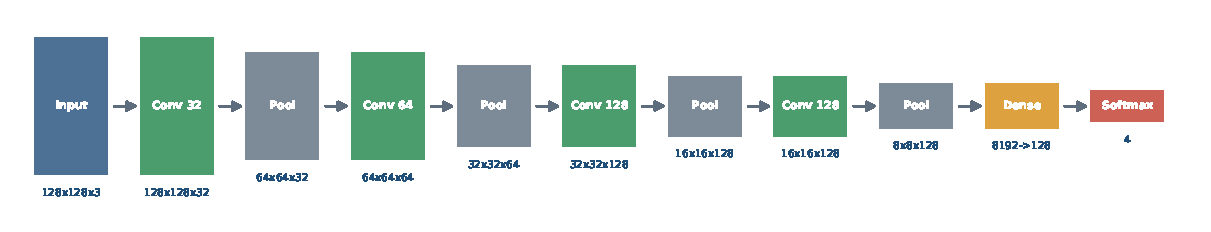
\includegraphics[width=\textwidth]{c1_pipeline.pdf}
\caption{Forward path of the reference network.}
\label{fig:pipeline}
\end{figure}

\begin{table}[tbp]
\centering
\caption{Layer-by-layer trace of a $128\times128\times3$ input. All
convolutions are $3\times3$ with $s=1$ and \emph{same} padding.}
\label{tab:trace}
\small
\begin{tabular}{llrr@{\hskip 0.8cm}llrr}
\toprule
\# & Layer & Output & Params & \# & Layer & Output & Params \\
\midrule
0 & Input    & $128^2\times3$  & 0        & 6 & MaxPool    & $16^2\times128$ & 0 \\
1 & Conv, 32 & $128^2\times32$ & 896      & 7 & Conv, 128  & $16^2\times128$ & 147{,}584 \\
2 & MaxPool  & $64^2\times32$  & 0        & 8 & MaxPool    & $8^2\times128$  & 0 \\
3 & Conv, 64 & $64^2\times64$  & 18{,}496 & 9 & Flatten    & 8192            & 0 \\
4 & MaxPool  & $32^2\times64$  & 0        & 10 & Dense, 128 & 128            & 1{,}048{,}704 \\
5 & Conv, 128 & $32^2\times128$ & 73{,}856 & 11 & Dense, 4  & 4              & 516 \\
\midrule
\multicolumn{8}{r}{\textbf{Total: 1{,}290{,}052 parameters}} \\
\bottomrule
\end{tabular}
\end{table}

Two patterns in Table~\ref{tab:trace} matter:

\begin{itemize}
  \item Spatial size falls while depth rises --- the network trades
  \emph{where} information is for \emph{what} it is.
  \item Parameters are very unevenly spread: four convolutional layers hold
  $19\%$ of the weights, while one dense layer holds $81\%$.
\end{itemize}

\subsection{Convolutional Layers}

A convolutional layer slides learnable \emph{kernels} across its input,
computing a dot product at each position \cite{lecun}:

\begin{equation}
y_{i,j,m} = b_m + \sum_{c=1}^{C_{\text{in}}}\sum_{u=1}^{K}\sum_{v=1}^{K}
w_{u,v,c,m}\,x_{\,i\cdot s+u,\;j\cdot s+v,\;c}
\end{equation}

This sum is the \emph{preactivation} $z$; applying
$\mathrm{ReLU}(z)=\max(0,z)$ gives the \emph{activation}.

\begin{figure}[tbp]
\centering
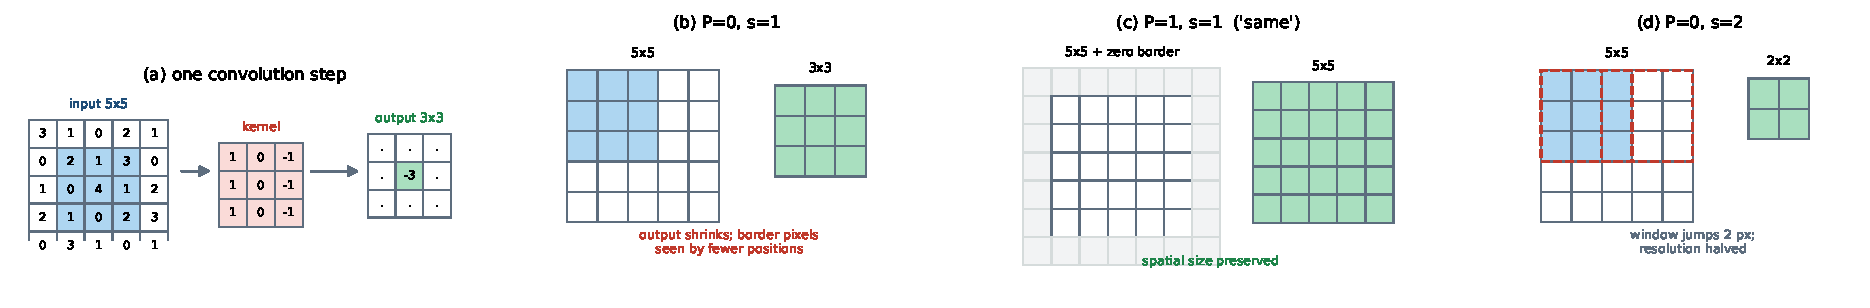
\includegraphics[width=\textwidth]{c2_conv.pdf}
\caption{(a) One convolution step: patch $\times$ kernel, summed, giving
$(2-3)+(0-1)+(1-2)=-3$. (b)--(d) Effect of padding $P$ and stride $s$ on a
$5\times5$ input with a $3\times3$ kernel.}
\label{fig:conv}
\end{figure}

The kernel in Figure~\ref{fig:conv}(a), with columns $[1,0,-1]$, fires where
intensity falls left to right --- a vertical edge detector. Nobody designed it;
it emerges because edges reduce the loss.

\begin{description}[leftmargin=2.0cm,style=nextline,itemsep=1pt]
  \item[Kernel size $K$] How much one neuron sees. Two stacked $3\times3$
  layers match one $5\times5$ layer using $18C^2$ weights instead of $25C^2$,
  plus an extra non-linearity.
  \item[Stride $s$] Step size of the window. $s=2$ halves resolution directly
  (Figure~\ref{fig:conv}d).
  \item[Padding $P$] Zero border. Without it the map shrinks and border pixels
  are visited from fewer positions (Figure~\ref{fig:conv}b). \emph{Same}
  padding, $P=(K-1)/2$, avoids both (Figure~\ref{fig:conv}c).
  \item[Channels $C_{\text{out}}$] Number of kernels, hence output depth. Each
  kernel spans \emph{all} input channels, so layer 1 holds
  $(3\!\cdot\!3\!\cdot\!3+1)\times32 = 896$ weights.
\end{description}

Output size follows from these:

\begin{equation}
H_{\text{out}} = \left\lfloor \frac{H_{\text{in}} - K + 2P}{s}\right\rfloor + 1
\end{equation}

Note what the 896 excludes --- the image resolution. That is the source of the
advantage in Section~\ref{sec:why-cnn}.

\textbf{Applications.} Any grid-structured signal: RGB images, multispectral
satellite bands, medical volumes, and with 1-D kernels, time series such as ECG
traces. AlexNet, VGG and ResNet are built from exactly these parts.

\subsection{Pooling and the Classification Head}

\begin{figure}[tbp]
\centering
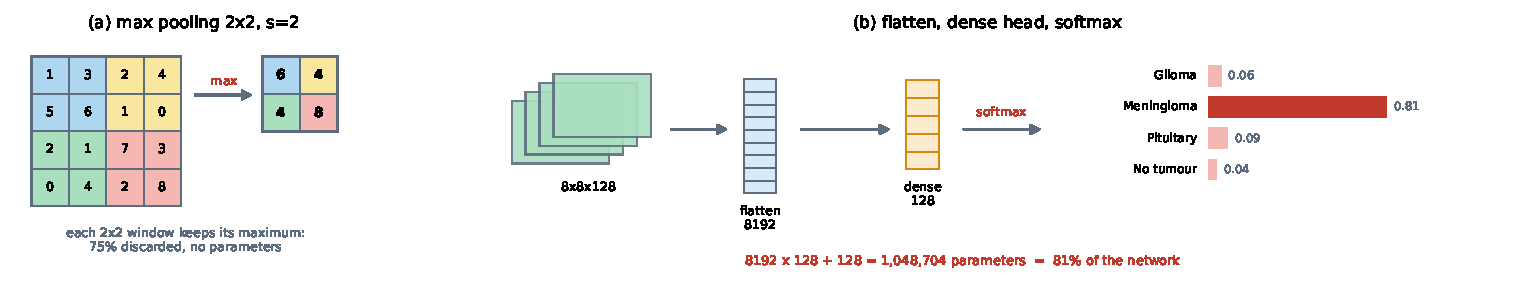
\includegraphics[width=\textwidth]{c3_pool_head.pdf}
\caption{(a) Max pooling, $2\times2$, stride 2. (b) Flatten, dense layer,
softmax.}
\label{fig:poolhead}
\end{figure}

\textbf{Pooling} replaces each neighbourhood with a summary statistic. Max
pooling keeps the largest activation and discards the rest
(Figure~\ref{fig:poolhead}a). It has no parameters and does three things:

\begin{itemize}
  \item Cuts the activation volume fourfold --- stage 2 of
  Table~\ref{tab:trace} reduces $524{,}288$ activations to $131{,}072$.
  \item Doubles the image area later kernels cover, reaching global context in
  fewer layers.
  \item Gives local translation invariance: a one-pixel shift inside a window
  leaves the maximum unchanged.
\end{itemize}

The cost is exact position, which suits classification but harms segmentation.

\textbf{The head} flattens the final volume and passes it through dense layers,
each computing $\mathbf{Z}=\mathbf{W}\mathbf{X}+\mathbf{b}$, with one output
unit per class. Softmax gives
$p(y=k\mid\mathbf{x}) = e^{z_k}/\sum_j e^{z_j}$, and training minimises
categorical cross-entropy:

\begin{equation}
\mathcal{L} = -\frac{1}{N}\sum_{i=1}^{N}\sum_{j=1}^{C} y_{ij}\log(p_{ij})
\end{equation}

So the conv stack is a learned \emph{feature extractor} and the head is a
\emph{classifier}. Flattening $8\times8\times128$ into 128 units costs
$1{,}048{,}704$ weights --- $81\%$ of the network. Two consequences:

\begin{itemize}
  \item Overfitting originates here, so dropout is applied here
  (Section~\ref{sec:dropout}).
  \item Stack and head are separable, so a pretrained stack can be reused with
  a fresh head --- transfer learning.
\end{itemize}

\subsection{Why CNNs Outperform Fully Connected Networks}
\label{sec:whycnn}
\label{sec:why-cnn}

A dense network can in principle represent anything a CNN can. The CNN's
advantage is \emph{inductive bias}: assumptions true of natural images, so a
smaller and better-aimed search space.

\begin{figure}[tbp]
\centering
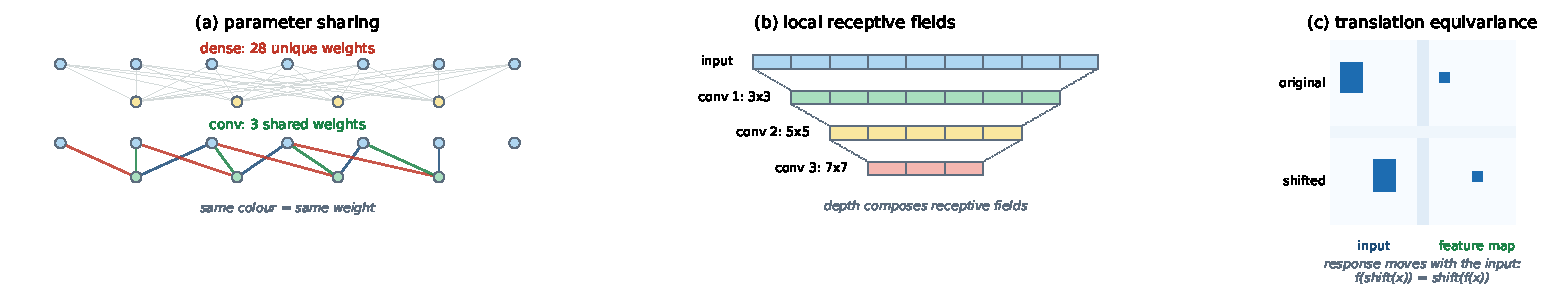
\includegraphics[width=\textwidth]{c4_why.pdf}
\caption{(a) One kernel reused everywhere. (b) Receptive fields composing with
depth. (c) A response that moves with its input.}
\label{fig:why}
\end{figure}

\textbf{Parameter sharing.} Dense layers give every connection a private
weight; convolution reuses one kernel everywhere. On this input a dense layer
of 512 units needs $128\cdot128\cdot3\cdot512+512 = 25{,}166{,}336$ parameters;
the convolutional layer that opens the network needs 896 --- about $0.004\%$ as
many. Fewer weights means
less capacity to memorise and a stronger gradient signal per weight.

\textbf{Local receptive fields.} Each neuron connects only to a small
neighbourhood, matching a real property of images: pixel correlation decays
with distance. A dense layer must instead \emph{learn} that distant pixels are
irrelevant. Long-range structure survives because receptive fields compose with
depth --- three stacked $3\times3$ layers give a $7\times7$ view.

\textbf{Translation equivariance.} Convolution commutes with translation:
$f(T_\delta \mathbf{x}) = T_\delta f(\mathbf{x})$. A detector learned in one
region works everywhere; a dense network must relearn a pattern for each
location. CNNs are often called translation \emph{invariant}. Strictly,
convolution is equivariant --- the response moves with the input. Invariance
belongs to the architecture as a whole, from equivariant convolutions plus
pooling discarding exact position.

Together these place the CNN at a better point on the bias--variance
trade-off: more constrained, with constraints correct for the domain.

\section{Theory II: Training and Generalisation}
\label{sec:theory2}

\subsection{Reading Loss Curves}

Training loss is measured on the data the optimiser updates on; validation loss
on held-out data producing no gradient updates \cite{goodfellow}.

\begin{figure}[tbp]
\centering
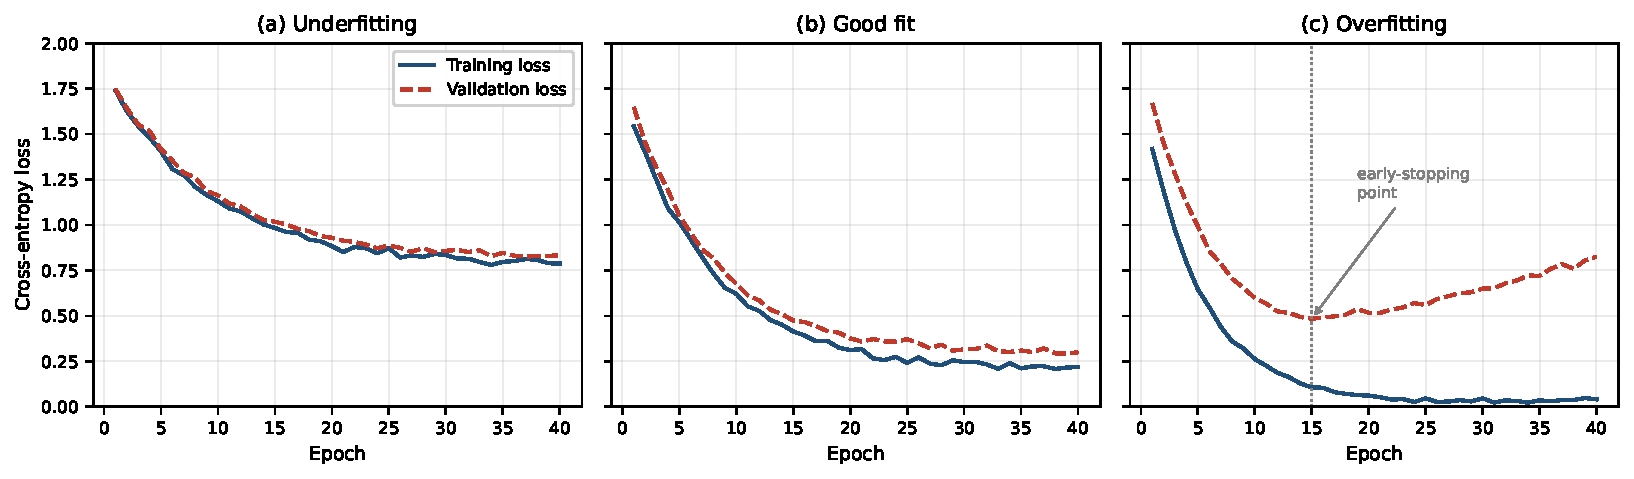
\includegraphics[width=\textwidth]{loss_curves.pdf}
\caption{The gap between curves measures variance; the height at which they
settle measures bias.}
\label{fig:curves}
\end{figure}

\begin{description}[leftmargin=2.9cm,style=nextline,itemsep=2pt]
  \item[Underfitting] Both losses flatten high, small gap. The model fails on
  data it has already seen, so more data will not help. Logistic regression on
  raw CIFAR-10 pixels stalls near $40\%$: a linear boundary in pixel space
  cannot separate the classes. Fix: more capacity, longer schedule, higher
  learning rate, weaker regularisation.
  \item[Good fit] Both fall, validation flattens slightly above training. A
  small gap is expected; what matters is that validation is flat, not rising.
  \item[Overfitting] Training loss $\to 0$ while validation bottoms out and
  climbs. The widening gap is the signature. Past the minimum the network
  memorises sensor noise, compression artefacts and incidental backgrounds.
  Typical trigger: a high-capacity CNN on a few thousand images, no
  augmentation.
\end{description}

Caution: validation loss \emph{below} training loss usually signals a bug ---
often dropout active in training but not validation.

\subsection{Dropout, Augmentation, Batch Normalisation}
\label{sec:dropout}

\textbf{Dropout} zeroes each unit with probability $p$ ($0.1$--$0.5$) every
forward pass, scaling survivors by $1/(1-p)$; at inference it is off. It
attacks \emph{co-adaptation} --- units forming fragile committees where one is
useful only because three specific others fire alongside it. Since no unit can
rely on a partner, each must learn an independently informative feature.
Equivalently, $n$ units define $2^n$ sub-networks sharing one weight set.
Applied in the dense head, where parameters concentrate.

\textbf{Data augmentation} applies label-preserving transforms on the fly. The
obvious effect is a larger training set; the important one is that it
\emph{states an invariance} the architecture does not encode. The transform set
is a modelling decision, not a default:

\begin{itemize}
  \item Satellite imagery has no canonical orientation --- flips and $90^\circ$
  rotations are valid, giving eight free variants per image.
  \item Traffic signs are the opposite: a vertical flip turns a left-turn arrow
  into a right-turn arrow while keeping the original label.
\end{itemize}

\textbf{Batch normalisation} normalises each channel per mini-batch, then
rescales with two learned parameters:

\begin{equation}
\hat{x}_i = \frac{x_i - \mu_B}{\sqrt{\sigma_B^2 + \varepsilon}},
\qquad y_i = \gamma \hat{x}_i + \beta
\end{equation}

Layer inputs shift during training because the layers beneath change
simultaneously. Fixing the first two moments stabilises this, allowing higher
learning rates and reducing sensitivity to initialisation. Standard placement
is \texttt{Conv $\to$ BatchNorm $\to$ ReLU}. At inference, running averages
replace batch statistics --- forgetting to switch to evaluation mode is a
common bug.

\begin{table}[tbp]
\centering
\caption{Regularisation methods and their mechanisms.}
\label{tab:reg}
\small
\begin{tabular}{ll}
\toprule
Method & Mechanism \\
\midrule
Dropout              & Randomly deactivates neurons during training \\
Batch normalisation  & Normalises activations per mini-batch \\
Layer normalisation  & Normalises across features; used in sequence models \\
Data augmentation    & Expands training data with label-preserving transforms \\
Weight decay ($L_2$) & Penalises large weight magnitudes \\
Early stopping       & Halts training at the validation minimum \\
\bottomrule
\end{tabular}
\end{table}

\subsection{Why a Separate Test Set Is Still Required}
\label{sec:testset}

The validation set stops being unbiased the moment it is used to make a
decision. No validation data enters the gradient computation --- but it is not
used once. It selects the learning rate, the architecture, whether augmentation
helped, the stopping epoch.

The optimiser fits the training set by gradient descent; the developer fits the
validation set by repeated selection. The mechanism differs, the consequence
does not.

\textbf{Example.} Twenty configurations, each truly $88\%$ accurate, with
validation accuracy fluctuating $\pm1.5$ points because the validation set is
finite. Taking the best of twenty reliably returns about $91\%$ --- three
points that are the maximum of twenty noisy draws, not a better model. The bias
grows with the number of configurations tried.

The test set is evaluated once, after every design decision is final. If a
disappointing test result prompts an architecture change, it has become a
validation set and its guarantee is gone. All model selection here uses
validation data alone; the test set is untouched until
Section~\ref{sec:results}.

\section{Dataset and Preprocessing}
\label{sec:data}

\textbf{Source, licence, size.} The four-class Brain Tumour MRI dataset
\cite{dataset} is a public Kaggle compilation of three upstream sources
(figshare, SARTAJ, Br35H), and neither MNIST nor FashionMNIST. The copy used
here holds $7{,}200$ images balanced at $1{,}400$ per class in
\texttt{Training/} and $400$ in \texttt{Testing/} --- a resampled variant of the
$7{,}023$ unbalanced upstream release, so every count below comes from the copy
actually used.

\textbf{Domain relevance.} Gliomas and meningiomas differ mainly in location and
margin character, and both can resemble normal tissue at low resolution. The
task therefore exercises sensitivity to local structure at an arbitrary
position --- what convolution supplies --- rather than rewarding a memorised
global template.

\textbf{Preprocessing.} An inventory pass found $75$ distinct image sizes, a
dominant $512\times512$ mode, and a mix of RGB and greyscale files. Scans are
cropped to the bounding box of non-background pixels --- much of each canvas is
black padding --- then resized to $128\times128$ and normalised with ImageNet
statistics. \texttt{Testing/} is read once, by \texttt{evaluate.py}; a
stratified $80/20$ split of \texttt{Training/} gives $4{,}480$ training,
$1{,}120$ validation and $1{,}600$ test images, augmentation applying to the
training subset only.

\subsection{An audit of the supplied split}
\label{sec:leakage}

The guarantee a held-out set provides (Section~\ref{sec:testset}) is a property
of the split, not of the folder names, so it was checked. Kapoor and Narayanan
\cite{kapoor} survey 294 papers across 17 fields and find leakage of this kind
to be a leading cause of irreproducible results, which is reason enough not to
take a shipped split on trust. Hashing \emph{file
bytes} reports zero duplicates spanning the two folders; hashing the
\emph{decoded pixels} gives a different answer, since the byte hashes differ
only because the copies were re-encoded. $114$ test images are pixel-identical
to a training image, verified at full resolution ($\max|\Delta| = 0$). Extending
this to near-duplicates by normalised cross-correlation of $64\times64$
thumbnails --- invariant to brightness and contrast --- flags $443$ of $1{,}600$
test images ($27.7\%$): $333$ \emph{notumor} ($83.2\%$ of the class), $103$
\emph{meningioma}, $7$ \emph{glioma}, $0$ \emph{pituitary}. Pituitary scoring
zero is the control that makes the measurement credible: the metric fires only
where duplicated scans exist, not on generic MRI similarity.

\begin{figure}[tbp]
\centering
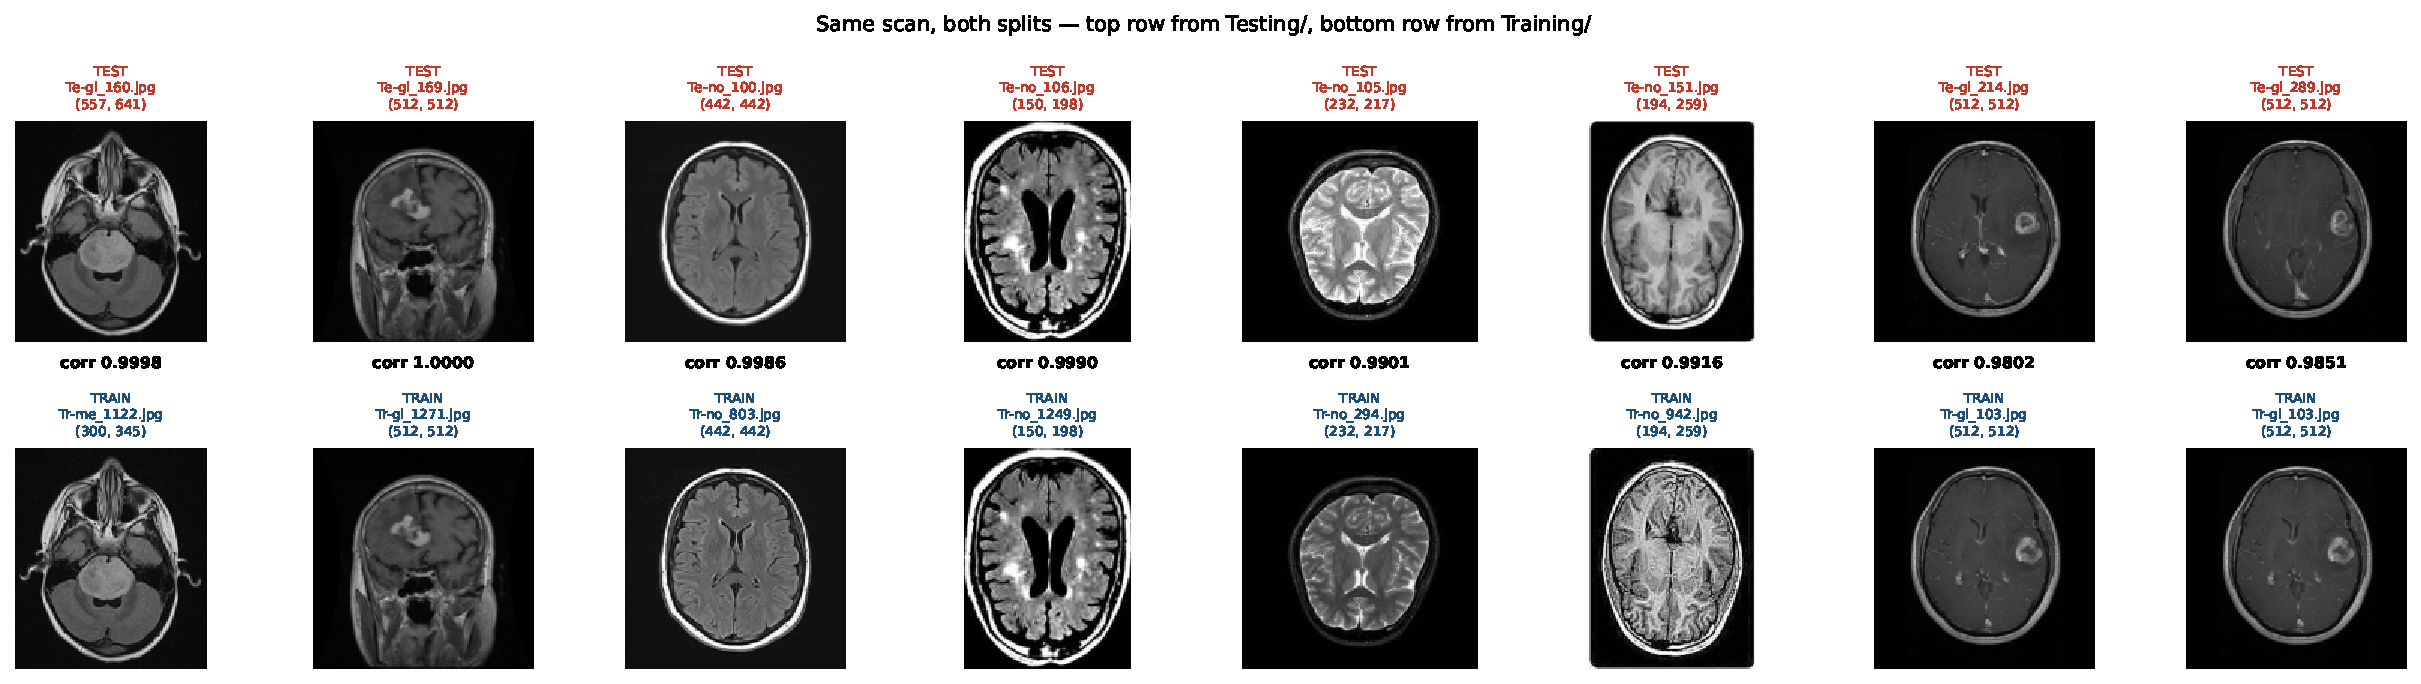
\includegraphics[width=0.95\textwidth]{res_leakage.pdf}
\caption{Scans present in both splits: top row from \texttt{Testing/}, bottom
from \texttt{Training/}, with the correlation between them. The rightmost pair
are adjacent slices of one patient rather than one scan duplicated.}
\label{fig:leak}
\end{figure}

Two further defects surfaced: two flagged pairs carry \emph{conflicting labels}
(one scan is glioma in \texttt{Testing/} and meningioma in \texttt{Training/} at
correlation $0.9998$, so at least one is wrong), and several pairs are adjacent
slices of one patient split across folders --- the patient-level leakage a
dataset without patient identifiers cannot be filtered for. All results below
are therefore reported over the full test set \emph{and} over the $1{,}157$
images with no training counterpart; the second is the defensible figure. A
smaller instance affects validation, where $187$ redundant copies within
\texttt{Training/} leave $59$ of $1{,}120$ validation images ($5.27\%$)
byte-identical to a training image.

%======================================================================
\section{Methodology}
\label{sec:method}

All three configurations share Adam at $10^{-3}$, batch size $32$,
cross-entropy loss, seed $42$, and early stopping on validation loss with
patience $8$; only architecture and augmentation vary, so each comparison
isolates one factor.

\textbf{Baseline.} A multilayer perceptron: flatten, one hidden layer of $512$
units with ReLU, dropout $0.5$, linear classifier --- $25{,}168{,}388$
parameters, $25.2$\,M in the first layer alone. Flattening destroys spatial
adjacency before the first weight is applied, so it has no locality, no
parameter sharing and no translation equivariance: the three properties of
Section~\ref{sec:whycnn}. Any gap is therefore attributable to those rather than
to capacity, the baseline carrying nineteen times more parameters than the model
that beats it.

\textbf{Improved CNN.} Four blocks of Conv--BatchNorm--ReLU--MaxPool with $32$,
$64$, $128$ and $128$ channels, then a dense head of $128$ units with dropout
$0.5$; $1{,}290{,}404$ parameters. \emph{$3\times3$ kernels throughout}
\cite{simonyan}: two stacked $3\times3$ layers span the same $5\times5$
receptive field using $18C^2$ weights rather than $25C^2$, with an extra
non-linearity between them. \emph{Same padding}, so border pixels are sampled as
often as central ones and downsampling happens only in the pooling layers, where
it is explicit. \emph{Channels double as resolution halves}, holding
representational capacity roughly constant while features grow more abstract.
\emph{BatchNorm before every activation} \cite{ioffe}, so the non-linearity
operates in a consistent range across batches; since it supplies its own shift,
the preceding convolutions are declared \texttt{bias=False}. \emph{Dropout only
in the head} \cite{srivastava}, which holds $81.3\%$ of the parameters and is
therefore where overfitting originates --- convolutional layers are already
regularised by weight sharing.

\textbf{Augmentation.}
\label{sec:aug}
Three transforms, applied to the training subset only, each stating an
invariance the architecture does not encode (Section~\ref{sec:dropout}; see
\cite{shorten} for a survey of the design space):
horizontal flip at $p=0.5$, since tumours occur in either hemisphere; rotation
of $\pm10^{\circ}$, since head positioning varies between patients while the
label does not; and brightness/contrast jitter of $\pm15\%$, since the three
upstream sources used different scanners, making intensity a nuisance variable.
Vertical flip is excluded --- anatomically implausible, it would assert an
invariance that is false. The effect is measured in Section~\ref{sec:quant}, not
assumed.

%======================================================================
\section{Results and Discussion}
\label{sec:results}

\begin{figure}[tbp]
\centering
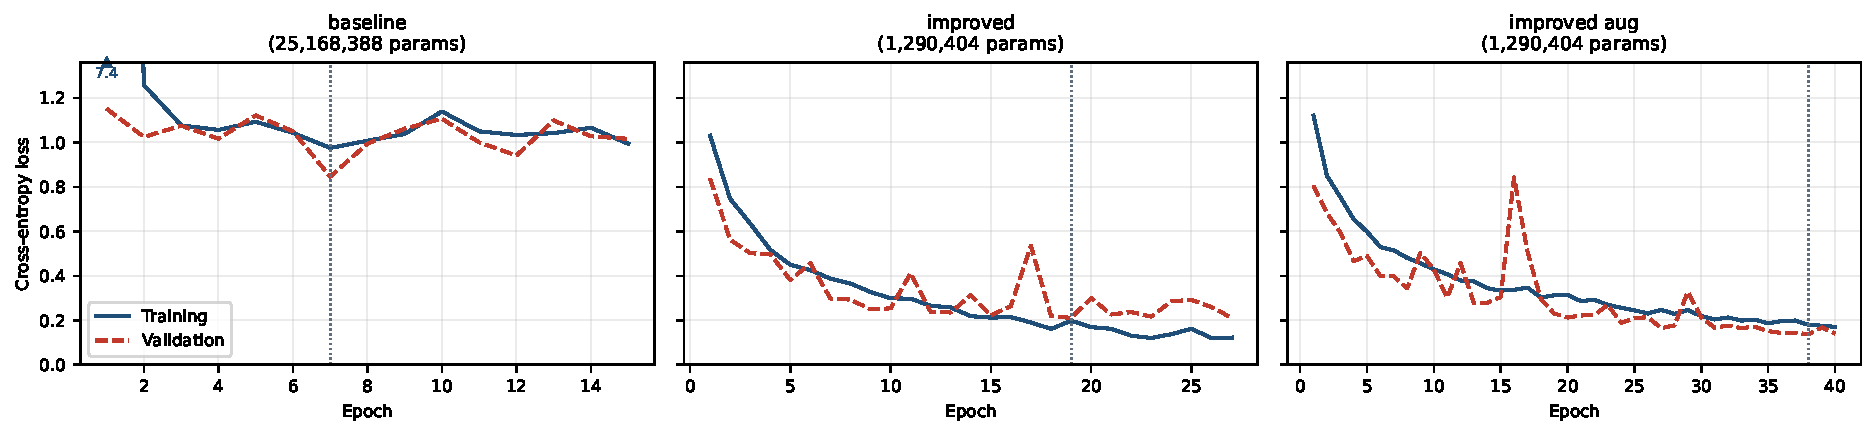
\includegraphics[width=\textwidth]{res_curves.pdf}
\caption{Training and validation cross-entropy; dotted line marks the
best-validation epoch. The baseline's first-epoch loss of $7.41$ is off-scale,
marked with a triangle.}
\label{fig:curves}
\end{figure}

\subsection{Learning-Curve Analysis}

The three panels correspond to the three regimes of
Section~\ref{sec:theory2}. The baseline \textbf{underfits}: both curves flatten
near a cross-entropy of $1.0$ with a small gap and stay there, early stopping
halting it at epoch $15$. Both losses high together is the diagnostic --- the
model fails on data it has already seen, so more data would not help. It is not
capacity-limited, having $19.5\times$ more parameters than the model that beats
it; it is structurally unsuited to the task. The un-augmented CNN begins to
\textbf{overfit}: training loss falls to $0.13$ while validation stalls near
$0.21$ and turns erratic after epoch $20$, the widening gap being the signature.
The augmented CNN shows a \textbf{good fit}: the curves track each other
throughout, validation sitting at or slightly below training --- consistent with
augmentation applying to the training subset alone, so training loss is measured
on a harder distribution. That run exhausted its $40$-epoch budget with its best
epoch at $38$, never triggering early stopping, so $91.2\%$ is a floor for the
configuration rather than its ceiling.

\subsection{Quantitative Comparison}
\label{sec:quant}

\begin{table}[tbp]
\centering
\small
\caption{Model comparison. \emph{Clean} is the $1{,}157$ test images with no
training counterpart (Section~\ref{sec:leakage}); macro F1 follows the same
column.}
\label{tab:results}
\begin{tabular}{lrrrrrr}
\toprule
& & & & \multicolumn{2}{c}{Test accuracy} & \\
\cmidrule(lr){5-6}
Configuration & Parameters & Epochs & Val. acc. & Full & \textbf{Clean} & Macro F1 \\
\midrule
Baseline (MLP)       & $25{,}168{,}388$ & 15/30 & 0.688 & 0.644 & --- & 0.641 \\
Improved CNN         & $1{,}290{,}404$  & 27/30 & 0.921 & 0.862 & --- & 0.860 \\
\quad + augmentation & $1{,}290{,}404$  & 40/40 & 0.952 & 0.912 & \textbf{0.902} & \textbf{0.866} \\
\bottomrule
\end{tabular}
\end{table}

Chance level for four balanced classes is $0.25$. \textbf{Architecture:} the CNN
improves test accuracy by $21.7$ points ($0.644 \rightarrow 0.862$) using
$19.5\times$ fewer parameters. Optimiser, schedule, data and augmentation are
identical across the two runs, so the difference is attributable to inductive
bias alone. \textbf{Augmentation:} with the architecture fixed, the policy of
Section~\ref{sec:aug} adds $5.0$ points of test accuracy and $3.0$ of validation
accuracy; its regularising effect is visible in Figure~\ref{fig:curves} as the
closed gap between the curves.

Excluding duplicated test images costs $1.0$ point of accuracy
($0.912 \rightarrow 0.902$) but $4.4$ of macro F1
($0.910 \rightarrow 0.866$), the contamination sitting almost entirely in one
class: only $67$ of $400$ \emph{notumor} test images survive the filter, and on
those its precision falls from $0.846$ to $0.568$. Its perfect recall over the
full test set is largely recall on images already seen, and the class is
effectively untestable here. On the clean subset glioma scores
$P\,0.981 / R\,0.784 / F1\,0.871$ ($n=393$), meningioma
$0.874 / 0.912 / 0.893$ ($n=297$) and pituitary $0.959 / 0.995 / 0.977$
($n=400$); the latter two barely move between columns, having almost no
contaminated images.

\subsection{Failure Cases and Improvement Ideas}

\begin{figure}[tbp]
\centering
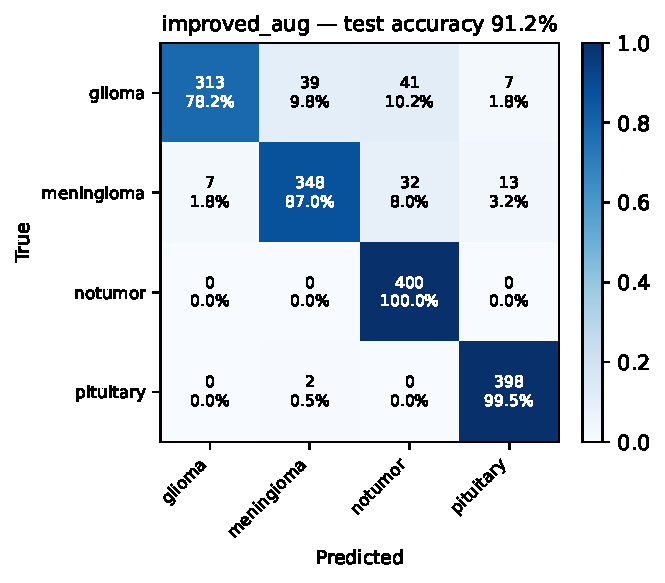
\includegraphics[width=0.60\textwidth]{res_confusion.pdf}
\caption{Confusion matrix over the full test set; rows are true classes. The
\emph{notumor} column absorbs $73$ scans from the two tumour classes, which is
the whole of its precision deficit.}
\label{fig:cm}
\end{figure}

\begin{figure}[tbp]
\centering
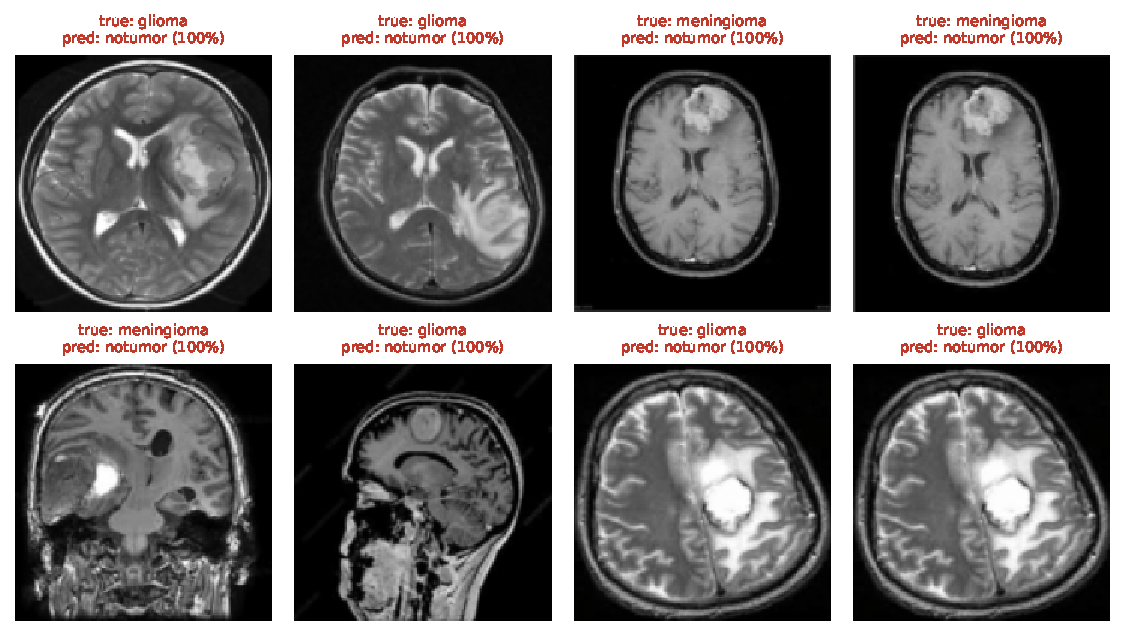
\includegraphics[width=0.92\textwidth]{res_failures.pdf}
\caption{The eight most confident misclassifications. Six are gliomas assigned
to \emph{notumor} at $100\%$ confidence, several of them showing a large and
visibly hyperintense lesion.}
\label{fig:fail}
\end{figure}

Of $141$ errors, $87$ are gliomas, splitting almost evenly between
\emph{notumor} ($41$) and \emph{meningioma} ($39$). \emph{Notumor} acts as a
sink: recall $1.000$, but the worst precision of the four classes, with $73$
scans from the tumour classes pulled into it. The direction matters clinically
--- $41$ of $400$ gliomas ($10.2\%$) are called healthy while the reverse error
never occurs. A model that never mistakes a healthy scan for a tumour but
discards one glioma in ten is optimised for the wrong asymmetry.

Figure~\ref{fig:fail} sharpens this: six of the eight most confident
errors are gliomas predicted \emph{notumor} at $100\%$ confidence, several
showing a large, visibly hyperintense lesion. A merely weak model produces
\emph{uncertain} errors; total confidence on an obvious lesion indicates either
a region of the input distribution never learned, or mislabelled source data ---
plausible here, since the upstream compilers documented replacing an unreliable
SARTAJ glioma folder and Section~\ref{sec:leakage} already found one provably
wrong label in this copy.

Four improvements follow, in order of expected return. \emph{Fix the split
first}: any gain measured on a $27.7\%$-contaminated test set is unverifiable,
so deduplicate at pixel level and re-split. \emph{Weight the loss towards glioma
recall}, or lower its decision threshold, trading notumor precision for the
error direction that matters at no architectural cost. \emph{Audit the glioma
labels}: if the confident failures are mislabelled, achievable recall exceeds
$0.784$. \emph{Transfer learning}: an ImageNet-pretrained backbone fine-tuned
here would likely beat a from-scratch $1.29$\,M network on $4{,}480$ images, at
the cost of the controlled comparison this report is built around.

%======================================================================
\section{Conclusion and Deployment Recommendation}
\label{sec:conclusion}

Both hypotheses held under controlled comparison: the CNN outperformed a fully
connected baseline by $21.7$ points of test accuracy using $19.5\times$ fewer
parameters, and augmentation added $5.0$ points more while visibly closing the
generalisation gap. The augmented CNN is the model to carry forward.

\textbf{It should not be deployed.} Three findings independently block that.
Glioma recall of $0.784$ means roughly one glioma in five is missed, and the
errors run in the clinically unsafe direction --- towards \emph{notumor}, never
away from it. The test split is $27.7\%$ contaminated, so even the corrected
$90.2\%$ rests on a dataset that cannot be fully audited and contains at least
one provably wrong label. And with no patient identifiers a patient-wise split
is impossible, so some optimism remains in any figure computed from it.

The defensible claim is narrower: on this data, convolutional inductive bias and
a modest augmentation policy together account for a $26.7$-point improvement
over a far larger fully connected model. That is a statement about architecture.
Clinical readiness would require a patient-wise split, a verified label set, and
a decision threshold tuned for the asymmetric cost of a missed tumour.

%======================================================================
\enlargethispage{3.5\baselineskip}
\section*{Reproducibility}

\small
Seeds are fixed at $42$ across Python, NumPy and PyTorch, with cuDNN
deterministic. Every figure and number in Sections~\ref{sec:data}
and~\ref{sec:results} is generated by the accompanying code and written to
\texttt{results/metrics.json} and \texttt{results/figures/}; none is transcribed
by hand. The test set is read once, by \texttt{evaluate.py}, after all three
models were trained. Runs used CPU (2 cores), PyTorch $2.13.0$, torchvision
$0.28.0$ and Python $3.11$, pinned in \texttt{requirements-lock.txt}; total
training time was $6{,}980$\,s. The pipeline reproduces by running
\texttt{notebooks/brain\_tumour\_cnn.ipynb} top to bottom.
\normalsize

% Repository: <URL>   <- re-add once the GitHub repo exists (+5 bonus)

%======================================================================
\enlargethispage{5\baselineskip}
\section*{Appendix A: Independent reproduction}

Console output from running \texttt{notebooks/brain\_tumour\_cnn.ipynb} end to
end on a second machine (Windows, Python 3.13, CPU) from the shipped
checkpoints; every quoted figure reproduces to four decimal places. The MLP
baseline is absent only because its checkpoint is $96$\,MB and is regenerated
rather than shipped.

\scriptsize
\begin{verbatim}
python 3.13.0  torch 2.13.0+cpu  torchvision 0.28.0+cpu  numpy 2.5.1  device cpu
scikit-learn 1.9.0  matplotlib 3.11.1  pillow 12.3.0

config          parameters   val acc  test acc  macro F1     (chance = 0.2500)
improved         1,290,404    0.9214    0.8619    0.8599
improved_aug     1,290,404    0.9518    0.9119    0.9103

improved_aug               n   accuracy   macro F1
full test set           1600     0.9119     0.9103
contaminated             443     0.9368
CLEAN (no train twin)   1157     0.9023     0.8663   (contamination 27.7%)
\end{verbatim}
\normalsize

\bibliographystyle{plain}
\begin{thebibliography}{9}
\footnotesize\setlength{\itemsep}{0pt}\setlength{\parskip}{0pt}
\bibitem{dataset} Nickparvar, M. (2021). \emph{Brain Tumor MRI Dataset}. Kaggle;
compiled from figshare, SARTAJ, Br35H.
\url{kaggle.com/datasets/masoudnickparvar/brain-tumor-mri-dataset}
\bibitem{ioffe} Ioffe, S. \& Szegedy, C. (2015). Batch normalization. \emph{ICML}.
\bibitem{srivastava} Srivastava, N. et al. (2014). Dropout. \emph{JMLR} 15(1), 1929--1958.
\bibitem{simonyan} Simonyan, K. \& Zisserman, A. (2015). Very deep convolutional
networks for large-scale image recognition. \emph{ICLR}.
\bibitem{lecun} LeCun, Y., Bottou, L., Bengio, Y. \& Haffner, P. (1998).
Gradient-based learning applied to document recognition. \emph{Proceedings of
the IEEE} 86(11), 2278--2324.
\bibitem{goodfellow} Goodfellow, I., Bengio, Y. \& Courville, A. (2016).
\emph{Deep Learning}. MIT Press.
\bibitem{shorten} Shorten, C. \& Khoshgoftaar, T. M. (2019). A survey on image
data augmentation for deep learning. \emph{Journal of Big Data} 6, article 60.
\bibitem{kapoor} Kapoor, S. \& Narayanan, A. (2023). Leakage and the
reproducibility crisis in machine-learning-based science. \emph{Patterns} 4(9),
100804.
\end{thebibliography}

\end{document}
